\section{Results}
\label{sec:results}

\begin{table}[t]
  \caption{RQ1 and RQ2, hand-picked sample: predicting hedge funds' quarterly trades, test period
  2022Q1--2026Q2 (\testrowsM{} positions). Fund acc.\ is accuracy averaged over funds; AUC ranks
  BUY against SELL from each model's continuous score. Foundation models are zero-shot on each
  position's share history. Best value in each column in bold.}
  \label{tab:rq1}
  \small
  \setlength{\tabcolsep}{3pt}
  \begin{tabular}{@{}lcccc@{}}
    \toprule
    Model & Accuracy & Macro-F1 & Fund acc. & AUC \\
    \midrule
    Majority class (per fund) & 56.4\% & 0.29 & 56.7\% & -- \\
    Recent majority (8 quarters) & 50.7\% & 0.42 & 52.9\% & -- \\
    Repeat last action & 44.1\% & 0.39 & 45.9\% & -- \\
    Rule: fund's net direction at $t-1$ & 51.1\% & 0.34 & 49.7\% & -- \\
    Logistic regression & 61.1\% & 0.45 & 58.8\% & 0.64 \\
    LSTM, 8-quarter sequences & 62.2\% & 0.46 & \textbf{61.3\%} & 0.65 \\
    LightGBM & \textbf{62.5\%} & \textbf{0.48} & 60.8\% & \textbf{0.66} \\
    \midrule
    Chronos-2, zero-shot & 58.3\% & 0.30 & 56.5\% & 0.57 \\
    \quad + returns, EPU covariates & 58.6\% & 0.31 & 56.5\% & -- \\
    TimesFM 2.5, zero-shot & 57.7\% & 0.30 & 54.7\% & 0.58 \\
    Chronos, finance-trained & 56.6\% & 0.25 & 56.7\% & 0.52 \\
    \bottomrule
  \end{tabular}
\end{table}


\subsection{RQ1: How predictable are hedge funds' trades?}

Hedge fund trades are only modestly predictable (Table~\ref{tab:rq1}).
LightGBM raises mean per-fund accuracy from \baseM\% for each fund's majority
action to \lgbM\%, a gain of \gainM{} points (95\% CI \gainloM{} to
\gainhiM{} when whole funds are resampled, and \twowayloM{} to \twowayhiM{}
when funds and quarters are resampled together). The gain is not luck:
it appears in all \dmposM{} test quarters (Diebold--Mariano $t = \dmtM$, $p <
0.001$; $t \geq \dmtminall$ in the other samples). The choice of model does not appear to
matter much. Logistic regression reaches \logitM\%, and an LSTM over each
position's last eight quarters, the model family of~\cite{cohen2026mimicking},
reaches \lstmM\%. The LSTM is slightly above LightGBM in per-fund accuracy but
below it on the other three metrics, so we report LightGBM; the conclusions
are the same with the LSTM. Simple rules are not able to beat the baseline, including
each fund's majority action over its last eight quarters (\recentM\%), because
hedge funds' overall direction changes from quarter to quarter. The model
relies mostly on fund identity, the position's weight and rank, and recent
fund activity, while past returns and peers' trades add little: what is
predictable is habit, not herding.

\begin{figure}[t]
  \centering
  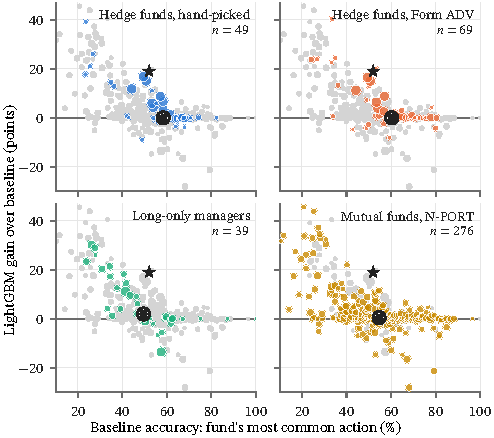
\includegraphics[width=0.92\linewidth]{figures/fig_rq1_funds.pdf}
  \caption{Each fund's gain from LightGBM over its own majority-class
  baseline (percentage points), against that baseline, one panel per sample
  ($n$: funds with test-period data; dot size: number of positions). Grey dots
  are the other samples' funds; ringed dots are sample medians; the line marks
  no gain. The star is the average over the mutual funds
  of~\cite{cohen2026mimicking} (52\% to 71\%), from a different period and data
  source, shown for reference only.}
  \label{fig:rq1}
\end{figure}

The average gain hides how it is spread across funds (Figure~\ref{fig:rq1}). For the median hedge fund the model adds \medgainM{} points, and
only \naboveM{} of \activeM{} funds gain more than one point. The gain comes
from the \nlowbaseM{} funds without a dominant action (baseline below 50\%),
where it is \gainlowbaseM{} points; for the rest it is \gainrestM{}. This is
not because large funds dominate the pooled training data: training with
equal total weight per fund gives a mean gain of \fundwtgainM{} and a median
of \fundwtmedM. Because hedge fund actions split almost evenly between BUY and
SELL, we also report measures that do not depend on the class mix. The model fixes
\errredM\% of the baseline's errors, lowers log-loss by \llskillM\% relative
to each fund's training class frequencies, and ranks a random BUY above a
random SELL with probability \aucbsM{}. Pooled accuracy (\lgbpooledM\%) is
higher because the somewhat more predictable multi-strategy and quantitative
funds supply \multiquantshareM\% of test positions.

These conclusions are robust (Table~\ref{tab:samples}). Under the rolling,
per-fund protocol of~\cite{cohen2026mimicking}, models trained separately for
each fund barely match the fund's majority action: LightGBM changes accuracy
by \protfundgainM{} points, a regularized logistic regression by
\protlogitgainM{} and an LSTM by \protlstmgainM{}. A single hedge fund's 20
quarters (a median of \medtrainM{} training cases) are too few and too
irregular to learn from; a pooled model retrained on each block's 20 quarters
gains \protpoolgainM. Dropping the rare HOLD class (BUY vs.\ SELL, \bsgainM{}
points, AUC \bsaucM{}) or widening the HOLD band to $\pm5\%$ (\hbgainM{})
still leaves small gains. Large trades are no easier: with a
$\pm25\%$ band the gain is \bigM{} points [\bigloM, \bighiM] (\bigerrM\% of
errors) for the hand-picked funds and \bigmin{} to \bigmax{} elsewhere, and
full exits are ranked with AUC \exitaucmin--\exitaucmax{} in every sample,
against \exitbasemin--\exitbasemax{} from each fund's exit rate alone.
Retraining every year on an expanding window raises accuracy by \yrdiffM{}
points (DM $p = \yrpM$), but the baseline rises too: the gain is \yrgainM{}
[\yrgainloM, \yrgainhiM] (\yrerrM\% of errors; \yrerrmin--\yrerrmax\% across
samples). Excluding the multi-strategy and quantitative
firms gives \exmqgain{} [\exmqlo, \exmqhi], and weighting each fund's
positions by their dollar value gives \dwgain{} [\dwlo, \dwhi]. 

\paragraph{Can the pipeline find predictability where it exists?} A negative
result only means something if the method could have found a positive one
(Table~\ref{tab:controls}). We make a random tenth or quarter of the funds
follow a simple rule on a visible feature, and the pipeline recovers the
attainable gain for those funds. Accuracy rises from \injbaseten\% to
\injmodelten\% for an exact rule, and from \injbasenoisy\% to
\injmodelnoisy\% (ceiling \injrulenoisy\%) when the rule holds for 80\% of
their positions. When the rule sets 55, 60 or 70\% of a fund's labels, it
recovers about \grrecsixty\% of the attainable gain, and the other funds are
unaffected.
Even rules worth only \weakattlo--\weakatthi{} points over the baseline
(5--30\% of labels) raise the model's gain on those funds above its gain on
the others in all \weakdraws{} draws (four rule strengths, three draws each;
averages \weakgainlo--\weakgainhi{} against \weakotherlo--\weakotherhi{} points).
Moreover, more history does not provide much benefit. Training on the last 6, 12 or 20
quarters before 2021 instead of all \lcallquarters{} gives gains of
\lcsixM{}, \lctwelveM{} and \lctwentyM{} points for the hand-picked hedge
funds (\lcallM{} with all quarters), \lcsixA{}, \lctwelveA{} and \lctwentyA{}
for the Form ADV funds, and \lcsixL{}, \lctwelveL{} and \lctwentyL{} for
long-only managers. Testing on an earlier period, 2017--2019, does not
raise it (\earlyM{} and \earlyA{} points for the hedge funds, \earlyL{} for
long-only managers). The pipeline is able to detect planted signals as small as the
real effect; real hedge fund trades carry little signal of this kind.

\begin{table}[t]
  \caption{Can the pipeline find predictability where it exists? Top: a random 10\% or 25\% of
  hand-picked funds is made to follow a visible rule (BUY if the stock's four-quarter momentum is
  positive), exactly or for 80\% of positions; mean test accuracy of those funds over 3 draws. Bottom:
  gain over the majority baseline (points, 95\% interval) when testing 2017--2019 (training
  2013Q3--2015) and with the best of 20 LightGBM configurations chosen on 2021. Equal entries in a row
  agree only after rounding (long-only: 6.18, 6.16, 6.19).}
  \label{tab:controls}
  \footnotesize
  \setlength{\tabcolsep}{3pt}
  \begin{tabular}{@{}lccc@{}}
    \toprule
    Injected funds & Baseline & Model & Rule (ceiling) \\
    \midrule
    10\% of funds, exact rule & 65.8\% & 100.0\% & 100.0\% \\
    10\% of funds, rule on 80\% & 59.0\% & 88.6\% & 88.6\% \\
    25\% of funds, exact rule & 65.5\% & 100.0\% & 100.0\% \\
    25\% of funds, rule on 80\% & 59.3\% & 88.2\% & 88.2\% \\
    \midrule
    Sample & Earlier period & Tuned & Main \\
    \midrule
    HF hand-picked & +0.6 [\ensuremath{-}1.0, 2.0] & +4.1 [2.0, 6.9] & +4.1 [1.8, 6.7] \\
    HF Form ADV & +2.0 [0.6, 3.5] & +3.6 [1.8, 5.6] & +3.5 [1.6, 5.6] \\
    Long-only & +6.2 [2.0, 11.7] & +6.2 [3.3, 9.6] & +6.2 [3.0, 9.5] \\
    \bottomrule
  \end{tabular}
\end{table}


\paragraph{Comparison with long-only managers and individual mutual funds.}
The same pipeline on the other samples (Table~\ref{tab:samples}) shows that
hedge funds do not appear to be particularly unusual. Active long-only managers hold far more HOLD
positions (\holdL\% of labels against \holdM\%), so repeating the last action
works for them. But the model's gain over the majority baseline is similar:
\gainL{} points [\gainloL, \gainhiL] and \errredL\% of errors fixed, against
\gainM{} [\gainloM, \gainhiM] and \errredM\% for hedge funds. The long-only
advantage over the hand-picked and Form ADV hedge funds, \diffgainM{}
[\diffgainloM, \diffgainhiM] and \diffgainA{} [\diffgainloA, \diffgainhiA]
points, is not significant (nor without the three ETF sponsors). This does not
prove they are equal: we rule out only a long-only advantage above
\diffgainhiM{} (hand-picked) or \diffgainhiA{} points (Form ADV). The key comparison uses individual
mutual funds, the unit of~\cite{cohen2026mimicking}. On \activeN{} active U.S.\
equity mutual funds from N-PORT, the model gains only \gainN{} points
[\gainloN, \gainhiN] and fixes \errredN\% of errors. Adding the same funds up
to their families gives \gainP{} [\gainloP, \gainhiP] and \errredP\%, not
significantly different from the funds that belong to these families
(\diffgainNP{} [\diffgainloNP, \diffgainhiNP]). Because N-PORT starts in late
2019, these models train on six quarters. Retraining every 13F sample on that
same window (Table~\ref{tab:samples}, ``same training window'' rows) gives a
consistent picture: gains of \shortgainM{} [\shortgainloM, \shortgainhiM] for
the hand-picked hedge funds (no longer significant), \shortgainA{} for the
Form ADV hedge funds and \shortgainL{} for long-only managers, fixing between
\shorterrmin{} and \shorterrmax\% of errors across all samples. In our
pipeline no group comes close to the 40\% of errors
that~\cite{cohen2026mimicking} fix for mutual funds over 1990--2023, adding
funds together does not significantly reduce predictability, and the earlier
2017--2019 period is no more predictable (Table~\ref{tab:controls}). The gap
with that study is therefore not specific to hedge funds. Our tests of
firm-level filings and of an earlier period use shorter training histories,
so they are less conclusive. Richer stock features do not close the gap: adding \firmn{} firm
characteristics raises the gain by at most \firmextramax{} points in any
sample (hand-picked: \firmextraM{} [\firmextraloM, \firmextrahiM], DM $p =
\firmdmpM$, Holm across samples \firmholmM), and no group fixes more than
\firmerrmax\% of errors. The gap most likely reflects the holdings data
(fund-level Morningstar holdings against public filings) and how much history
each fund has.

\begin{table*}[t]
  \caption{The five samples under the identical pipeline. Funds: in the sample (active in the test
  period 2022Q1--2026Q2). Accuracy is mean per-fund accuracy; gains are in points over each fund's
  majority action, with 95\% intervals from resampling funds. The 13F samples train on 2013Q3--2020Q4;
  N-PORT begins in late 2019, so the ``same training window'' rows retrain every sample on
  2020Q1--2021Q2 (validation 2021H2) for a like-for-like comparison. The per-fund protocol
  of~\cite{cohen2026mimicking} (20 training and 8 test quarters, four blocks 2018Q3--2026Q2, one model
  per fund, gains over the same blocks' majority baseline) needs 28 quarters and is not available for N-PORT.}
  \label{tab:samples}
  \small
  \setlength{\tabcolsep}{4pt}
  \begin{tabular}{@{}lccccc@{}}
    \toprule
     & \multicolumn{2}{c}{Hedge funds (13F)} & Long-only & \multicolumn{2}{c}{Mutual funds (N-PORT)} \\
    \cmidrule(lr){2-3} \cmidrule(lr){5-6}
     & Hand-picked & Form ADV & managers (13F) & Individual funds & Fund families \\
    \midrule
    Funds (active in test) & 49 (49) & 99 (69) & 57 (39) & 300 (276) & 59 (53) \\
    \quad SELL/BUY/HOLD (\%) & 49/48/2 & 49/48/3 & 40/37/23 & 49/31/20 & 49/34/17 \\
    Test cases & 100,935 & 99,002 & 57,486 & 286,154 & 139,892 \\
    Training window & 2013Q3--20Q4 & 2013Q3--20Q4 & 2013Q3--20Q4 & 2020Q1--21Q2 & 2020Q1--21Q2 \\
    \midrule
    Majority baseline & 56.7\% & 59.4\% & 49.7\% & 53.7\% & 54.0\% \\
    Gain [95\% CI] & +4.1 [1.8, 6.7] & +3.5 [1.6, 5.6] & +6.2 [3.0, 9.5] & +2.9 [1.9, 4.0] & +2.2 [0.5, 4.2] \\
    Baseline errors fixed & 9\% & 9\% & 12\% & 6\% & 5\% \\
    Fund-weighted training, gain & +2.6 & +2.7 & +6.4 & +2.6 & +2.3 \\
    BUY vs.\ SELL only, gain & +2.7 & +0.7 & +2.1 & -- & -- \\
    HOLD band $\pm5\%$, gain & +2.3 & +3.2 & +5.8 & -- & -- \\
    \midrule
    Per-fund protocol of~\cite{cohen2026mimicking}: LightGBM & \ensuremath{-}1.1 & \ensuremath{-}1.1 & +0.5 & -- & -- \\
    \quad logistic regression & \ensuremath{-}1.9 & -- & -- & -- & -- \\
    \quad LSTM & +0.7 & -- & -- & -- & -- \\
    \quad pooled LightGBM & +2.5 & +2.3 & +4.4 & -- & -- \\
    \midrule
    Same training window: gain & +1.8 [\ensuremath{-}0.7, 4.4] & +3.3 [1.5, 5.3] & +4.7 [0.1, 9.0] & same as above & same as above \\
    \quad errors fixed & 4\% & 8\% & 9\% & same as above & same as above \\
    \midrule
    Oracle (fund's direction at $t$), gain & +3.0 & +4.5 & +2.9 & +5.2 & +0.7 \\
    LightGBM + oracle, gain & +7.0 & +7.2 & +10.9 & +8.6 & +4.6 \\
    \bottomrule
  \end{tabular}
\end{table*}


\subsection{What drives the low predictability?}

\emph{Fund-wide direction versus stock selection.} Much of a fund's quarterly
behavior could be fund-wide: flows, changes in gross exposure, de-risking. An
oracle that is told each fund's actual net direction in quarter $t$ and
predicts it for every position gains only \oraclegainM{} points, less than the
model. Adding the fund's actual quarter-$t$ buy share to LightGBM as a feature
raises the gain to \lgboraclegainM{} points (\lgboracleM\% accuracy), still
far below the mutual-fund benchmark (Table~\ref{tab:samples};
\lgboraclegainA{}, \lgboraclegainL{}, \lgboraclegainN{} and
\lgboraclegainP{} points in the other four samples). Even when the fund's
overall direction is known, which of its stocks it buys or sells remains
largely unpredictable.

\emph{Private information and aggregation.} If hedge funds traded on private
information, their trades should be least predictable in smaller, more opaque
stocks, and more so than long-only managers' trades. The gain in the smallest
third of the universe relative to the largest is \smlM{} points [\smlloM,
\smlhiM] for the hand-picked hedge funds, but \smlA{} for the Form ADV funds
and \smlL{} for long-only managers; the hedge-fund minus long-only difference
is \smldiffM{} [\smldiffloM, \smldiffhiM]. If netting across a firm's many
portfolios blurred predictability, funds with more positions would be less
predictable. Instead, the rank correlation between a fund's gain and its
number of holdings is \rhoholdingsM{} [\rhoholdingsloM, \rhoholdingshiM]
(\rhoholdingsA{} Form ADV, \rhoholdingsL{} long-only). Neither simple
explanation singles out hedge funds.

\subsection{RQ2: Do foundation models and news help?}

Used zero-shot, none of the three foundation models beats the majority
baseline in mean per-fund accuracy (Table~\ref{tab:rq1}). Chronos-2 reaches
\chronosM\% (\chronosDM\% with return and policy-uncertainty covariates),
TimesFM~2.5 \timesfmM\%, and the Chronos model pre-trained only on U.S.\
stock returns up to 2020 \fintextM\%, against \baseM\% for the baseline. On a
pooled accuracy basis, which favors large funds, Chronos-2 is able to beat the majority
baseline (\chronospooledM\% against \basepooledM\%). Diebold--Mariano tests find Chronos-2 and TimesFM significantly worse than the
baseline ($t = \dmtchronos$ and $\dmttimesfm$) and the finance-trained Chronos
not different from it ($p = \dmpfintext$). Their tuned cut-offs collapse to a
single threshold, so they never predict HOLD. Judged by ranking
instead, which does not depend on cut-offs, their scores carry some
information (BUY-vs-SELL AUC \aucchronosM, \auctimesfmM{} and \aucfintextM),
but less than LightGBM (\auclgbM). Position histories are short (a median of
\medhistM{} quarters), jumpy and driven by decisions rather than dynamics,
unlike the series these models learn from~\cite{rahimikia2025tsfm}. By
comparison, the LSTM in Table~\ref{tab:rq1}, a small model trained on the
holdings sequences themselves, does better than all three.

\begin{table}[t]
  \caption{RQ2: change in mean per-fund accuracy (points) when each input is added to LightGBM,
  hand-picked sample, with 95\% intervals from resampling funds (2,000 draws). News inputs are
  tested on 2022--2023, the test years with news data.}
  \label{tab:rq2}
  \small
  \setlength{\tabcolsep}{4pt}
  \begin{tabular}{@{}llc@{}}
    \toprule
    Added input & Years & Change [95\% CI] \\
    \midrule
    Chronos-2 forecast & 2022--26 & +0.49 [0.08, 0.99] \\
    TimesFM forecast & 2022--26 & +0.13 [$-$0.16, 0.43] \\
    News, previous quarter ($t-1$) & 2022--23 & $-$0.23 [$-$0.79, 0.31] \\
    \quad last 15 days of $t-1$ only & 2022--23 & $-$0.36 [$-$0.96, 0.25] \\
    News, same quarter ($t$) & 2022--23 & $-$0.50 [$-$1.17, 0.16] \\
    \quad last 15 days of $t$ only & 2022--23 & $-$0.12 [$-$0.50, 0.29] \\
    Chronos-2 + all news & 2022--23 & $-$0.16 [$-$0.72, 0.29] \\
    \bottomrule
  \end{tabular}
\end{table}


As extra inputs they help little (Table~\ref{tab:rq2}; the finance-trained
Chronos covers only the validation and test years, so it cannot be used as a
training feature). Adding the Chronos-2 forecast to LightGBM raises accuracy
by \rqtwochronos{} points [\rqtwochronoslo, \rqtwochronoshi]. This is the only
interval in Table~\ref{tab:rq2} that excludes zero (unadjusted for
multiplicity), and the gain disappears in the 2022--2023 subperiod; TimesFM
adds \rqtwotimesfm{} [\rqtwotimesfmlo, \rqtwotimesfmhi]. News does not help,
whether from the previous quarter (a forecast), from the same quarter (a
nowcast made before the filing is public), or only from the last 15 days
before quarter-end. No interval reaches beyond \rqtwomaxhi{} points, which
is small next to the model's own gain over the majority baseline in the same
2022--2023 window (\newswindowgain{} points [\newswindowlo, \newswindowhi]).
The LLM's reading of the news does not help either (\rqtwollmprev{} and
\rqtwollmnow{} points; Table~\ref{tab:rq2}). Its outlook's rank correlation
with next-quarter market-adjusted returns is \llmmemnamed{} with the name
shown and \llmmemanon{} hidden (gap $t = \llmmemt$, $p = \llmmemp$): the
name changes some answers, but even named outlooks do not predict returns.

\subsection{RQ3: Do unpredicted trades earn more?}

\begin{table}[t]
  \caption{RQ3: return spreads before disclosure, from the end of quarter $t$ to the day each
  fund's 13F for $t$ became public (at most 45 days), in excess of the average universe stock;
  \% per window, averaged over \rqthreequartersM{} quarters (Newey--West $t$). Primary tests show Holm-adjusted
  $p$-values within each sample in brackets. Positive values mean surprising trades did better.}
  \label{tab:rq3main}
  \footnotesize
  \setlength{\tabcolsep}{1pt}
  \begin{tabular}{@{}lccc@{}}
    \toprule
     & \multicolumn{2}{c}{Hedge funds} & Long-only \\ \cmidrule(lr){2-3}
     & Hand-picked & Form ADV & managers \\
    \midrule
    \multicolumn{4}{@{}l}{\emph{Primary}} \\
    Sells (pred. $-$ surpr.) & +0.43 (3.3) [0.013] & +0.33 (1.4) [0.532] & +0.33 (1.4) [0.582] \\
    \quad Holm over all nine & [0.038] & [1.000] & [1.000] \\
    Buys (surpr. $-$ pred.) & +0.17 (0.7) [0.927] & \ensuremath{-}0.02 (\ensuremath{-}0.1) [1.000] & +0.24 (0.9) [0.582] \\
    Stocks (Q1 $-$ Q5) & \ensuremath{-}0.21 (\ensuremath{-}0.6) [0.927] & \ensuremath{-}0.19 (\ensuremath{-}0.5) [1.000] & \ensuremath{-}0.56 (\ensuremath{-}1.2) [0.582] \\
    \multicolumn{4}{@{}l}{\emph{Secondary}} \\
    All buys $-$ sells & +0.16 (1.3) & +0.16 (1.5) & \ensuremath{-}0.20 (\ensuremath{-}1.4) \\
    Sells, size--mom. adj. & +0.31 (1.9) & +0.25 (1.3) & +0.12 (0.8) \\
    Sells, intensity & +0.46 (1.6) & +0.16 (0.8) & +0.37 (1.4) \\
    Sells, within fund & +0.50 (1.0) & \ensuremath{-}0.35 (\ensuremath{-}0.7) & +0.43 (0.9) \\
    Sells, after filing & +0.31 (1.8) & +0.01 (0.0) & \ensuremath{-}0.07 (\ensuremath{-}0.2) \\
    Buys, after filing & +0.20 (1.0) & \ensuremath{-}0.14 (\ensuremath{-}0.7) & +0.46 (1.8) \\
    \bottomrule
  \end{tabular}
\end{table}


Our primary test uses the window in which only the fund knew its trades: from
the end of quarter $t$ to the day its 13F for $t$ became public (a median of
\filinglagmedian{} days; only \filedthirtyone\% of hedge fund reports appear
within a month), over \rqthreequartersM{} formation quarters
(2022Q1--2026Q2). Because the model is barely better than each fund's
majority action, a ``surprise'' here is mostly a trade against the fund's
usual direction. Table~\ref{tab:rq3main} reports three primary spreads (in \%
over the window; positive means the surprising trades did better), with
Holm-adjusted $p$-values within each sample and across all nine primary tests. In
the hand-picked sample the sell spread is \pdsellsM\%: stocks the funds sold
unexpectedly did worse than stocks they sold as predicted ($t =
\pdsellstM$; Holm $p = \pdsellsholmM$ within the sample and
\pdsellsholmallM{} across samples). This holds even when every trade without
a price is treated as a delisting that loses 30\% (\pdsellsdlM\%). But the
spread is smaller after matching each stock to universe stocks of the same
size and momentum tercile (\pdsellschM\%, $t = \pdsellschtM$), and it does not
replicate in the Form ADV sample (\pdsellsA\%, $t = \pdsellstA$) or among
long-only managers (\pdsellsL\%, $t = \pdsellstL$). Comparing a fund's
surprise sells only with its own predicted sells in the same quarter gives a
similar point estimate but much less precision (\wfsellsM\%, $t =
\wfsellstM$), so we cannot tell whether the spread reflects which funds are
selling or which stocks they sell. Sells against a fund's overall direction
resemble the discretionary, valuation-motivated trades
that~\cite{alexander2007motivation} find informative for mutual funds.
Surprise buys and the stock-level spread show no edge in any sample, and
neither do sorts on the model's probability of the action taken (surprise
intensity). Across all trades, the funds' buys do not beat their sells over the window
(\pduncondM\% and \pduncondA\% for the two hedge fund samples). For a copier,
who can trade only after the filing, the three months after disclosure show
no significant spread (sells \cpsellsM\%, $t = \cpsellstM$; buys
\cpbuysM\%, $t = \cpbuystM$).

Following~\cite{cohen2026mimicking} more closely at the
manager level, a fund's predictability gain is unrelated to the payoff of its
trades before disclosure (rank correlation \mgrrhoM{} [\mgrloM, \mgrhiM]
across \mgrnM{} hand-picked funds; \mgrrhoA{} and \mgrrhoL{} in the other
samples).

A calendar-time version over the three months after quarter-end, which spans
disclosure, agrees. The surprise-sells spread is \rawsells\% per month raw
($t = \rawsellst$) and \ffsells\% ($t = \ffsellst$) after the five
Fama--French factors and momentum. Across weightings and holding periods of up
to 12 months (Newey--West lags equal to the holding period), \rqthreesig{} of
24 overlapping, exploratory specifications reach $|t| \geq 1.96$. The hand-picked
sell spread exceeds the Form ADV one by \diffsamplesells\% per month ($t =
\diffsamplesellst$). On the other hand, funds in both samples and funds only in the
hand-picked one have similar spreads (\overlapsells\% and
\nonoverlapsells\%), so the gap does not come from hand-picking winners.

These tests have limited power. In the calendar-time version, the smallest
monthly alpha we could detect with 80\% power is \trademdelo--\trademdehi\%
for the trade-level spreads and \stockmdeM\% for the stock-level spread. For
the stock-level spread, where~\cite{cohen2026mimicking} report a five-factor
alpha of 3.86\% per year (0.32\% per month) for mutual funds, our 95\%
intervals are [\stockciloM, \stockcihiM] (hand-picked) and [\stockciloA,
\stockcihiA] (Form ADV), in \% per month, so we cannot rule out an effect of
that size. Our conclusion is narrow: apart from one result for surprise sells
that is specific to the hand-picked sample and weakens with size and momentum
matching, any extra return to unpredicted 13F trades is statistically
indistinguishable from zero over this window.
